%%%%%%%%%%%%%%%%%%%%%%%%%%%%%%%%%%%%%%%%%%%%%%%%%%%%%%%%%%%%%%%%%%%%%%%%
\chapter{Introduction}
%%%%%%%%%%%%%%%%%%%%%%%%%%%%%%%%%%%%%%%%%%%%%%%%%%%%%%%%%%%%%%%%%%%%%%%%

\section{Context: Network Analysis}
\label{sec:intro:context}

Most complex systems and phenomena are amenable to be modeled as graphs as they
consist of entities interacting with each other.
%
Think of the network of computers exchanging data between them that form the
Internet, the (virtual) friendships among the users of a social network, the
power grids connecting generating facilities to electrical substations, or the
biochemical interactions happening in a biological cell.
Often, the analysis of the patterns of relationships of a network
(also known as network analysis) reveals interesting insights about the
underlying system~\cite{DBLP:conf/cscw/BackstromK14,
DBLP:conf/dsc/ZuoZ16,tang2012inferring,lambiotte2008geographical}.
Today, network analysis is an established scientific field aiming to unveil
non-trivial properties of complex systems by analyzing the structure of their
interconnections.

Network analysis emerged from graph theory, whose roots date back in the early
\nth{18} Century when the Seven Bridges of K\"onigsberg
problem\footnote{A recreational activity for the residents of K\"onigsberg was
to determine whether one could cross all the seven bridges of the city exactly
once and, if possible, return to their starting point.} was modeled as a graph
and resolved (negatively) by the Swiss mathematician Leonhard Euler.
Graph theory continued to develop and started to be applied to other areas
such as chemistry or social sciences.
In particular, thanks to the great interest that graph theory sparked among social
scientists, the \nth{20} Century witnessed the development of Social Network
Analysis (SNA), a discipline that investigates social ties between individuals
through the use of graphs.

The idea of looking at society in terms of interconnections among
social actors was first conceived by the French philosopher Auguste Comte~\cite[p.
14]{DBLP:journals/socnet/Bernard05}. Only in the 1930s, however, the group led
by the Romanian-American psychologist Jacob Levy Moreno developed the first
\emph{sociograms}~\cite{moreno1934shall} (\ie graphic representations of social
ties between people) as well as an approach that includes all the defining
properties of social network analysis. As argued by Freeman: \enquote{It was
based on structural intuitions, it involved the collection of systematic
empirical data, graphic imagery was an integral part of its tools and it
embodied an explicit mathematical model.}~\cite[p. 39]{DBLP:journals/socnet/Bernard05}.

In this thesis, we address two popular problems that, among others, immediately
found applications in the context of social networks and were later applied to
many other fields beyond SNA~\cite{DBLP:journals/jis/OtteR02}: (i) identifying the
individuals that are the most \enquote{important} according to some criterion
and (ii) matching each individual (or as many as possible) with the best
suitable candidate -- also known as the maximum (weighted) matching problem.

Centrality measures -- \ie functions that assign to each vertex (or edge) of a
network an importance score -- turned out to be a successful technique to
identify important individuals in a social network.
Centrality stems from the concept of \emph{centralization}, devised for the
first time in the late 1940s thanks to experiments aimed to study communication
patterns and group collaboration conducted at MIT by Alex Bavelas's
group~\cite{bavelas1948mathematical}.
Results suggested that centralization is related to a group's efficiency in terms of
problem-solving capabilities~\cite[p. 45]{trahair1994aristotelian} and agreed
with the perception of influence of each individual
actor~\cite[p. 68]{DBLP:journals/socnet/Bernard05}. These experiments led to
the definition of
\emph{closeness centrality}\footnote{Closeness is one of the
oldest centrality measures; it is defined as the reciprocal of farness, \ie
the sum of shortest-path distances from an actor to all the others.}
in 1950~\cite{bavelas1950communication} and, in the following decades, to the
development of many other centrality indices that have been employed in
a multitude of applications far beyond SNA.
Examples include the control of epidemic
spreading~\cite{DBLP:journals/snam/Doostmohammadian20}, the study of the
political integration of Indian social life~\cite{cohn1958networks} or even the
analysis of the centralization of political parties and elite networks in the
\nth{15} Century Florence to explain the power of the Medici
family~\cite{action1993rise}.
% Write a bit more about different centrality measures?

The maximum weighted matching problem (or MWM), in turn, derives from the
well-studied Stable Roommates Problem (SRP). SRP was first introduced in the
seminal work by Gale and Shapley in 1962 as a variation of the famous Stable
Marriage Problem~\cite{DBLP:journals/tamm/GaleS13} and appears in numerous
practical applications~\cite{iwama2007stable}.
In its most basic form, SRP takes as input a set of participants, with each one
having ranked the others in order of preference.
The desired output is a \emph{stable} matching (\ie a separation of the set into
disjoint pairs of \enquote{roommates}); a matching is stable if
there are no two participants that prefer to be matched
together rather than with their current matching partner.
Among all the possible stable matchings in a network, however, some
applications require to find the one with maximum weight,\footnote{The weight
of a matching $M$ is defined as the sum of the edge weights in $M$.}
hence the maximum weighted matching problem.
Examples include information retrieval~\cite{DBLP:conf/ecir/LaitangPB13},
pattern recognition~\cite{DBLP:journals/ijprai/ConteFSV04},
multilevel graph partitioning~\cite{DBLP:journals/pc/MonienPD00}, and many
others~\cite{wang2004bipartite,DBLP:conf/ismb/BorgwardtOSVSK05,
DBLP:journals/dc/HalldorssonKPR18,DBLP:journals/jpdc/Patt-ShamirRS12}.
As of today, MWM is one of the most popular combinatorial optimization
problems~\cite{DBLP:journals/networks/Johnson94,DBLP:journals/eatcs/Manlove14,
bisseling2020parallel}.


\section{Motivation}
\label{sec:intro:motivation}
%
\paragraph{Centrality in Large-Scale Networks}
%
Traditionally, centrality measures have been applied to graphs
with relatively small size.
In the last decades, however, factors such as the increasing computing power of
modern machines, the rapid growth of the Internet and of
online social networks, automatic data collection and many others catalyzed
the rapid growth (both in size and quantity) of graph datasets.
Hence, massive networks with millions to billions of vertices and edges are now
ubiquitous.
Computing (even in approximation) traditional centrality measures in such large
graphs is challenging as many of them inherently have a high computational
complexity or are averse to approximation schemes or require operations that
are not amenable to
parallelization~\cite{DBLP:conf/sdm/KangPST11}.

A goal of this work is to develop \emph{scalable}
algorithms for centrality computation in large real-world networks.
The term \enquote{scalability}
refers here to the capability of an algorithm to process massive data sets in
reasonable time. Usually, this implies that the time complexity is (nearly-)linear
in the input size. We do not refer in this context to \emph{parallel} scalability
(\ie the capability of an algorithm to use multiple processors to execute faster),
although in some cases we exploit shared-memory or even distributed-memory
parallelism to speed our algorithms up.
Our algorithms achieve scalability through three strategies: \emph{approximation}
(\ie yielding inexact result\change{s} with bounded errors),
\emph{heuristics} (\ie yielding inexact solutions without error bounds), and by
\change{devising and} computing new centrality
measures that are more amenable to scalability than traditional ones.

\Cref{ch:electrical-closeness} provides an example of approximation: we present
a fast algorithm to approximate electrical closeness as well as other electrical
centrality measures.
Because computing electrical closeness exactly is prohibitive
on large graphs, we introduce a new sampling-based approach that yields results
with higher quality (in terms of maximum absolute error) and \change{is} faster
compared to state-of-the-art algorithms. This enables for the first time the
possibility to approximate electrical closeness on graphs with hundreds of
millions of vertices in minutes.

Concerning heuristics, \Cref{ch:group-closeness-local-search} introduces
new local search algorithms for group-closeness maximization, \ie
the problem of finding a set of $k$ vertices with highest group-closeness
centrality.\footnote{Group-closeness is a set function that measures
the centrality of a group $S\subset V$ of vertices according to
the average shortest-path distance from $S$ to the vertices outside $S$.
See \Cref{eq:def:dist-point-set} for the distance between a vertex and a set of
vertices.} This problem is \np-hard and there is no algorithm known to
solve it exactly in reasonable time on graphs with more than a few thousands of
vertices.
In a matter of seconds, our heuristics compute high-quality solutions on
networks with hundreds of millions of vertices -- instead of several hours with
existing algorithms.

Because shortest-path based measures are inherently expensive to compute,
\change{we propose, in \Cref{ch:ged-walk},} an alternative (algebraic) group
centrality measure inspired by Katz centrality (see \Cref{eq:def:katz}) that is
based on \emph{walks} of any length instead of shortest paths. Our experiments
suggest that not only our new measure can be \change{maximized (in approximation)}
faster than existing group centralities, but it also improves the precision of
popular graph mining tasks to a greater extent \change{than} existing measures.

\paragraph{Dynamic Graphs}
%
Networks often evolve over time, \change{creating} new connections or deleting existing
ones.
Changes can happen very frequently:
consider the frenetic activity on social media platforms or the emails that
are sent every second.\footnote{See \url{https://www.internetlivestats.com}.}
For these \emph{dynamic} networks, analyzing each snapshot independently
(\eg by running a static algorithm after every single update) is clearly an
inefficient choice, especially for rapidly-changing networks.
This raises the need for more effective approaches tailored to dynamic graphs.

Thus, another objective of this work is to design scalable dynamic algorithms
capable of efficiently recomputing the required information after one or
multiple changes occur.
In particular, we develop algorithms to efficiently maintain in a dynamic graph: (i)
the ranking of the top-$k$ vertices with highest closeness
centrality (\Cref{ch:dyn-topk}) and a $\change{(1/2)}$-approximation of the MWM
(\Cref{ch:dyn-mwm}).

\section{Methodology}
\label{sec:intro:methodology}
%
\begin{figure}[t]
\centering
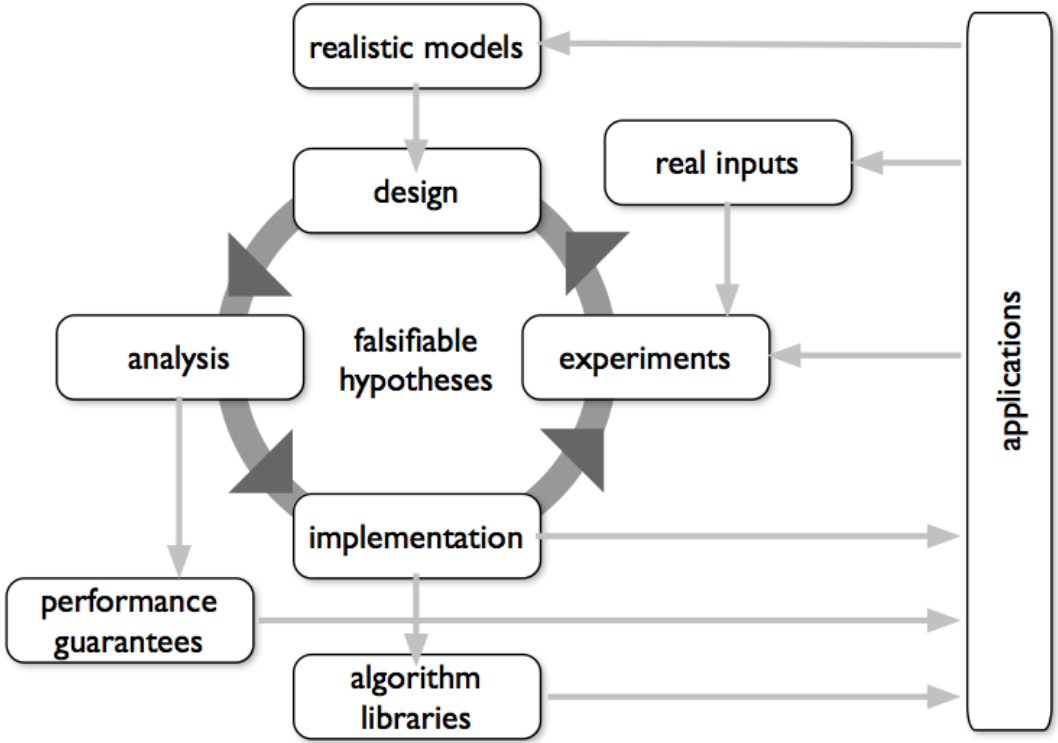
\includegraphics[width=.65\textwidth]{sources/figures/ae.png}
\caption{Algorithm Engineering schema~\cite{DBLP:conf/birthday/Sanders09}.}
\label{fig:intro:algo-eng}
\end{figure}

\paragraph{Algorithm Engineering}
The algorithmic contributions presented in this thesis were developed following
the \emph{algorithm engineering} paradigm.
Algorithm engineering can be summarized as a feedback loop of five
iterative phases: (i) modeling the problem, which usually stems from
practical applications, (ii) designing an algorithm, (iii)
analyzing it theoretically, (iv) implementing it, and (v) evaluating it
via systematic experiments (\ie experimental algorithmics), see
\Cref{fig:intro:algo-eng} for an overview.
The process is cyclic rather than sequential because experimental results
shall unveil insights about that problem that lead to further (theoretical)
improvements of the algorithms.
According to this paradigm, the implementation and the experimental evaluation
of an algorithm are not left to practitioners but are part of the whole
development process. Hence, all the algorithms presented in this thesis
are implemented in practice and evaluated on real-world instances;
in particular, they are implemented in C++ as part of the open-source
NetworKit~\cite{DBLP:journals/netsci/StaudtSM16} library.

\paragraph{Experimental Algorithmics}
As described above,
experimental evaluation is a crucial step of the algorithm engineering process.
In particular, to effectively support our conclusions, it is essential to
implement a systematic and reproducible experimental pipeline.
To this end, our experiments follow, when applicable, the guidelines for
experimental algorithmics presented in
Ref.~\cite{DBLP:journals/algorithms/AngrimanGLMNPT19} -- which I
coauthored. In particular, we carefully select appropriate sets of instances
(both real-world and synthetic) belonging
to different classes.\footnote{Although there are several ways to categorize a
network~\cite{DBLP:journals/algorithms/AngrimanGLMNPT19},
in this work, we \change{often refer to the class of \emph{complex} networks.}
As the name suggests, complex networks present non-trivial (complex)
topological features, most notably: a small diameter (\emph{small-world}
effect~\cite{newman2018networks}), clustering (\ie the tendency of vertices to
form densely connected clusters), and a skewed degree distribution
(many vertices with low degree and a few vertices with high
degree)~\cite{DBLP:journals/corr/cond-mat-0106096}.
Simple networks \change{such as road
networks or random graphs (\eg graphs generated by the \erdosr model)
do not present such features}.}
We always obtain real-world instances from public repositories (\eg
KONECT~\cite{kunegis2013konect}, SNAP~\cite{snapnets}, and others) whereas for
synthetic instances we provide details about the graph generators we used.
Also, we make our code publicly available as part of the NetworKit toolkit.
The reproducibility of our experiments is guaranteed by
managing them with SimexPal~\cite{DBLP:journals/algorithms/AngrimanGLMNPT19},
a software that automates the experimental pipeline and simplifies gathering
and analyzing the results according to the
guidelines~\cite{DBLP:journals/algorithms/AngrimanGLMNPT19}.

\section{Outline and Contribution}
%
This work is structured into five parts.
The first one provides a broad overview of the addressed network-analytic
challenges and fundamental notation and definitions,
\Crefrange{part:single-vertex-centrality}{part:matching} present in detail our
algorithmic contributions, and \Cref{part:conclusion} is devoted to concluding
remarks.
More precisely, \Cref{part:single-vertex-centrality} focuses on computing
and approximating popular single-vertex centrality measures.
In \Cref{part:group-centrality}, we consider \emph{group-centrality}, \ie the
concept of centrality extended to groups of vertices as described by
Everett and Borgatti~\cite{everett1999centrality}; in particular, we introduce
approximation algorithms and fast heuristics for group centrality maximization.
Finally, \Cref{part:matching} presents a batch-dynamic algorithm that maintains
\change{a} $\change{(1/2)}$-approximation of an MWM in fully-dynamic graphs.

The contributions presented in this thesis appeared in the publications
reported in \Cref{apx:publications}; in the following, we provide a detailed
overview.

\paragraph{\Cref{part:single-vertex-centrality}: Algorithms for Single-Vertex
Centrality Measures}
%
Centrality measures are widely used to quantify the importance of single
vertices on the basis of their structural position in a network. Concerning closeness,
Bergamini \etal~\cite{DBLP:journals/tkdd/BergaminiBCMM19} introduced an
efficient algorithm to identify the top-$k$ vertices with highest closeness
centrality that, in practice, is much faster than computing the closeness of
all vertices and extracting the top-$k$ ranking later. On dynamic graphs, however, it
would anyway be too costly to run this algorithm after each edge update (or
batch of updates). Hence, in \Cref{ch:dyn-topk}, we propose a batch-dynamic
algorithm for updating the top-$k$ ranking after multiple edge updates. Our algorithm
is developed upon the existing static strategy by Bergamini
\etal~\cite{DBLP:journals/tkdd/BergaminiBCMM19}. Experiments show that, for
single edge updates and for batches with up to $100$ edge updates, our dynamic
algorithm is one to four orders of magnitude faster than the static one.

In \Cref{ch:betweenness-approx}, we consider the problem of implementing an
effective parallelization strategy for adaptive sampling and we apply it to
betweenness centrality approximation as a case study.
%Approximation algorithms trade solution quality to reduce running time in order
%to provide solutions faster than an exact computation. In this chapter, we focus
%on \emph{adaptive sampling} algorithms.
Adaptive sampling algorithms draw random samples according to an
algorithm-specific distribution and aggregate them.
A \emph{stopping condition} determines whether enough samples have been drawn --
thus the name \enquote{adaptive}. Because the stopping condition requires to
evaluate all the data generated so far, parallelization strategies for
adaptive sampling algorithms are challenging to devise. In addition,
evaluating the stopping condition is often not cheap (\eg for our
betweenness case study, it is linear in the number of vertices of the graph);
hence, there is a trade-off between (i) frequently checking the stopping condition,
which implies additional time overhead (but avoids drawing many samples in
excess) and (ii) checking the stopping condition less frequently (with a
higher risk of drawing many samples in excess).
We introduce a new epoch-based parallelization framework for adaptive sampling
that avoids expensive synchronization costs. The main idea is to split the
execution of each thread into discrete \emph{epochs}. During an epoch, each
thread draws samples; the stopping condition is checked only at the end of
each epoch and always by the same thread, while the others keep drawing samples
for the next epoch. In this way, threads do not idle while the stopping
condition is being checked.
We adapt this framework to \kadabra, the state-of-the-art algorithm for
betweenness approximation. Our interest in \kadabra stems from the fact that
this algorithm implements an adaptive sampling technique but it fails to scale
to large numbers of threads due to high synchronization costs. We propose three
algorithms that achieve different trade-offs in terms of memory footprint and
determinism of the results. Furthermore, we use parameter
tuning~\cite{DBLP:journals/algorithms/AngrimanGLMNPT19} to optimize the
frequency of checking the stopping condition.
Our experimental study shows that our framework achieves much better parallel
speedups compared to a straightforward OpenMP-based parallelization strategy
for \kadabra.

Finally, \Cref{ch:electrical-closeness} targets the problem of approximating
\emph{electrical} centrality measures, especially electrical closeness and
forest closeness. These measures interpret the underlying graph as an
electrical network (with edge weights representing the resistance between
two vertices) and the distance between two vertices $u$ and $v$ is
computed as the resulting resistance between them (\ie the \emph{effective
resistance} or resistance distance, see \Cref{sec:prelim-resistance-distance}).
Resistance distance \change{and forest distance} consider \emph{all} the paths
between $u$ and $v$, not only the shortest ones.
%
Unfortunately, existing methods to compute electrical closeness and forest
closeness exactly rely on computing the pseudoinverse \Linv of the Laplacian
matrix \Lapl (see \Cref{sec:prelim-graphs}), which is prohibitive in terms of
both time and memory -- typically, \Linv is dense.
We present a new efficient sampling-based strategy that only requires a linear
amount of additional memory and exploits two main properties:
(i) the resistance distance between any two vertices only requires an arbitrary
column and the diagonal of \Linv (not the whole matrix) and (ii) the resistance
distance of an edge $e$ is proportional
to the fraction of the spanning trees that contain $e$. Our algorithm
provides a probabilistic $\pm\epsilon$-approximation of
\diag{\Linv} by solving just one Laplacian system
and by sampling a fixed amount of uniform spanning trees.
Experimental results show that, compared to state-of-the-art strategies,
our algorithm not only is much faster and more memory-efficient, but also
yields much more accurate approximation of \diag{\Linv} in terms of absolute
error, which results in more precise complete rankings of the elements
of \diag{\Linv}.


\paragraph{\Cref{part:group-centrality}: Algorithms for Group Centrality Measures}
%
Group centrality is useful for applications seeking sets of vertices that are
central \emph{as a group} rather than the top most individually central
vertices. Examples include finding the $k$ most influential actors in a social
network to promote some product or idea~\cite{DBLP:journals/toc/KempeKT15} or
placing resources among $k$ peers in a large P2P network so that they are
easily accessible by others~\cite{DBLP:journals/pe/GkantsidisMS06}.

Unfortunately, finding the most central group of $k$ vertices is an \np-hard
problem for most group centrality measures. This leaves approximation
algorithms and heuristics the only viable options for instances with more than
a few thousand vertices. Yet, existing algorithms for group centrality
maximization have limitations: (i) they fail to scale to large networks and, in
the group-closeness case, (ii) they do not provide any approximation guarantee.
Moreover, existing measures are not suitable for disconnected graphs. In this
part, we propose solutions to these issues.

In \Cref{ch:group-closeness-local-search,ch:ged-walk}, we target the lack of truly
scalable algorithms for group centrality maximization from two different
directions.
More precisely, \Cref{ch:group-closeness-local-search} focuses exclusively on
group-closeness: The fastest existing algorithm for this problem is the greedy
ascent heuristic by Bergamini \etal~\cite{DBLP:conf/alenex/BergaminiGM18}, which needs
several hours to handle graphs with hundreds of millions of edges.
We introduce a family of novel local search heuristics that require no more
than a few minutes to handle even larger graphs while yielding solutions with
nearly the same quality.
The fact that group-closeness is based on shortest paths poses
complexity-theoretic limitations to the development of scalable approximation
algorithms to maximize this measure. This motivates us to approach this problem
from a different angle, that is, introducing an alternative measure.
\Cref{ch:ged-walk} introduces GED-Walk (for \emph{Group Exponentially Decaying
Walk}), a novel group centrality measure inspired by Katz centrality. Similarly
to Katz, it takes into account \emph{walks} of any length -- with shorter walks
being more relevant than longer ones.
We present algorithms to compute and maximize (in approximation) GED-Walk.
On real-world networks and for groups with up to 100 vertices, our maximization
algorithm for GED-Walk is up to two orders of magnitude faster than state-of-the-art
\change{greedy} maximization algorithms for group-betweenness,
\change{group-closeness, and group-harmonic}.
%
\Cref{ch:ged-walk} also targets the lack of electrical
group centrality measures for disconnected graphs by introducing
group forest closeness, \ie forest
closeness\footnote{Forest closeness (see \Cref{sec:centrality-measures})
is an electrical centrality measure designed to handle disconnected graphs.}
extended to sets of vertices, and by adapting the greedy maximization algorithm
by Li \etal~\cite{DBLP:conf/www/0002PSYZ19} to group forest closeness.
Our experiments also show that, in connected graphs, the precision of
popular graph mining applications can be improved by GED-Walk to a greater
extent compared to other measures.
Analogous results are achieved in disconnected graphs by group forest closeness.

\Cref{ch:group-harm-clos-max} deals with approximating
group-closeness maximization. Building on top of the theoretical results
achieved in Ref.~\cite{DBLP:conf/alenex/AngrimanBDGGM21}, we present
the first approximation algorithm for this problem.
%In this chapter, we also address the issue of group centrality in disconnected
%graphs: we introduce group-harmonic closeness, \ie harmonic
%closeness\footnote{Harmonic closeness (see \Cref{sec:centrality-measures})
%handles disconnected graphs out of the box as it considers the harmonic sum
%of the distances from a vertex (or a set of vertices) to the others.}
%extended to groups of vertices, as well as a greedy approximation algorithm
%to maximize group-harmonic.
A clear trade-off between solution quality and running time emerges from our
experiments: our approximation algorithms consistently find higher quality
solutions compared to existing approaches at the cost of additional running
time.

\paragraph{\Cref{part:matching}: Maximum Weighted Matching in Fully-Dynamic Graphs}
%
On dynamic graphs, updating a previously computed matching after each
update (or a batch of updates) is a more efficient approach than
re-running a static algorithm from scratch -- similarly to what we observe in
\Cref{ch:dyn-topk} for the top-$k$ closeness centrality ranking.
%
Despite the wide range of algorithms for dynamic maximum (weighted) matching
proposed in the literature, little effort was invested into implementing these
algorithms in practice and evaluating their performance on real-world
instances. Only recently, implementations and experimental analyses were
done by Henzinger \etal~\cite{DBLP:conf/esa/Henzinger0P020} for dynamic maximum
cardinality matching algorithms and in
Ref.~\cite{conf/acda/AngrimanMSU21} for dynamic MWM -- which I coauthored.
These algorithms efficiently update an approximate maximum (weighted) matching
after single edge updates.

In \Cref{ch:dyn-mwm}, we consider the problem of maintaining a
$\change{(1/2)}$-approximate MWM after \emph{multiple} edge updates, as applications
dealing with rapidly-evolving networks may not require to compute a solution for
every single snapshot of the graph -- \eg self-organizing LTE
networks~\cite{DBLP:journals/cm/HuZZYW10}.
We take inspiration from the state-of-the-art \suitor algorithm by
Manne and Halappanavar~\cite{DBLP:conf/ipps/ManneH14}.
Our dynamic strategy is \change{conceptually} similar to the one implemented for
top-$k$ closeness in \Cref{ch:dyn-topk}: we use \suitor to compute an approximate MWM
on an initial snapshot of the graph; then, after one or multiple edge updates,
we identify the affected vertices (\ie the ones whose matching partner
needs to be updated) and update their matching partner accordingly.
Although in a worst-case scenario every vertex is affected by a single update
(which implies that our dynamic algorithm has the same \change{worst-case}
time complexity than the static \suitor), in our experiments, we see that the
actual number of affected vertices is very small -- it grows at most linearly
with the batch size. For single edge updates, our dynamic approach is on
average faster \change{than} the state of the
art~\cite{conf/acda/AngrimanMSU21}\change{,} whereas for batches with up to
$10^4$ edge updates it is two to six orders of magnitude faster than a static
recomputation (Ref.~\cite{conf/acda/AngrimanMSU21} only supports single edge
updates).
